\documentclass[10pt]{article}

% Lines beginning with the percent sign are comments
% This file has been commented to help you understand more about LaTeX

% DO NOT EDIT THE LINES BETWEEN THE TWO LONG HORIZONTAL LINES

%---------------------------------------------------------------------------------------------------------

% Packages add extra functionality.
\usepackage{
	times,
	graphicx,
	epstopdf,
	fancyhdr,
	amsfonts,
	amsthm,
	amsmath,
	algorithm,
	algorithmic,
	xspace,
	hyperref}
\usepackage[left=1in,top=1in,right=1in,bottom=1in]{geometry}
\usepackage{sect sty}	%For centering section headings
\usepackage{enumerate}	%Allows more labeling options for enumerate environments
\usepackage{epsfig}
\usepackage[space]{grffile}
\usepackage{booktabs}
\usepackage{amsmath}
\usepackage[super]{nth}

% This will set LaTeX to look for figures in the same directory as the .tex file
\graphicspath{.} % The dot means current directory.

\pagestyle{fancy}

\lhead{\YOURID}
\chead{\MyLang: Language Specification}
\rhead{\today}
\lfoot{CSCI 334: Principles of Programming Languages}
\cfoot{\thepage}
\rfoot{Spring 2020}

% Some commands for changing header and footer format
\renewcommand{\headrulewidth}{0.4pt}
\renewcommand{\headwidth}{\textwidth}
\renewcommand{\footrulewidth}{0.4pt}

% These let you use common environments
\newtheorem{claim}{Claim}
\newtheorem{definition}{Definition}
\newtheorem{theorem}{Theorem}
\newtheorem{lemma}{Lemma}
\newtheorem{observation}{Observation}
\newtheorem{question}{Question}

\setlength{\parindent}{0cm}
%---------------------------------------------------------------------------------------------------------

% DON'T CHANGE ANYTHING ABOVE HERE

% Edit below as instructed
\newcommand{\YOURID}{Hugo Hua}	% Replace "Your Name Here" with your name
\newcommand{\MyLang}{blueberry}	% Replace MyLang with your language name #
\newcommand{\ProblemHeader}	% Don't change this!

\begin{document}

\vspace{\baselineskip}	% Add some vertical space

% Refer to the lab handouts to determine what should go in each of these sections.  Each lab is additive.  So lab 8 should include everything you wrote in lab 7.  Lab 9 should include everything you wrote in lab 8, etc.

\section{Introduction}
This language is used to write sheet music for guitar tabs. Maybe in the future it'll be able to write normal sheet music as well! \\
I've always found GUI music writing software to be annoying to use, and it's always difficult to find all the buttons and features you need. I've felt like it would be easier and faster to simply type out music, since typing something like 'e4' is faster than looking for the right buttons and finding the right placement. This language would also be very customizable, and the user could adjust widths, spacing, etc.


\section{Design Principles}
I want the language to be as simple and intuitive as possible. The syntax is very simple, and a lot of the formatting is taken care of by the evaluator, which means that there are default values for a lot of parameters, making life easier for the user. Aesthetically, I'm working to make sure the output sheet music follows music engraving standards to look professional.


\section{Example Programs}
Minimal example:

\begin{verbatim}
-type tab
-time 4-4
-key c

1: 
   3e4
   4g
   1g
2:
   5a
   1f

\end{verbatim}


Output:

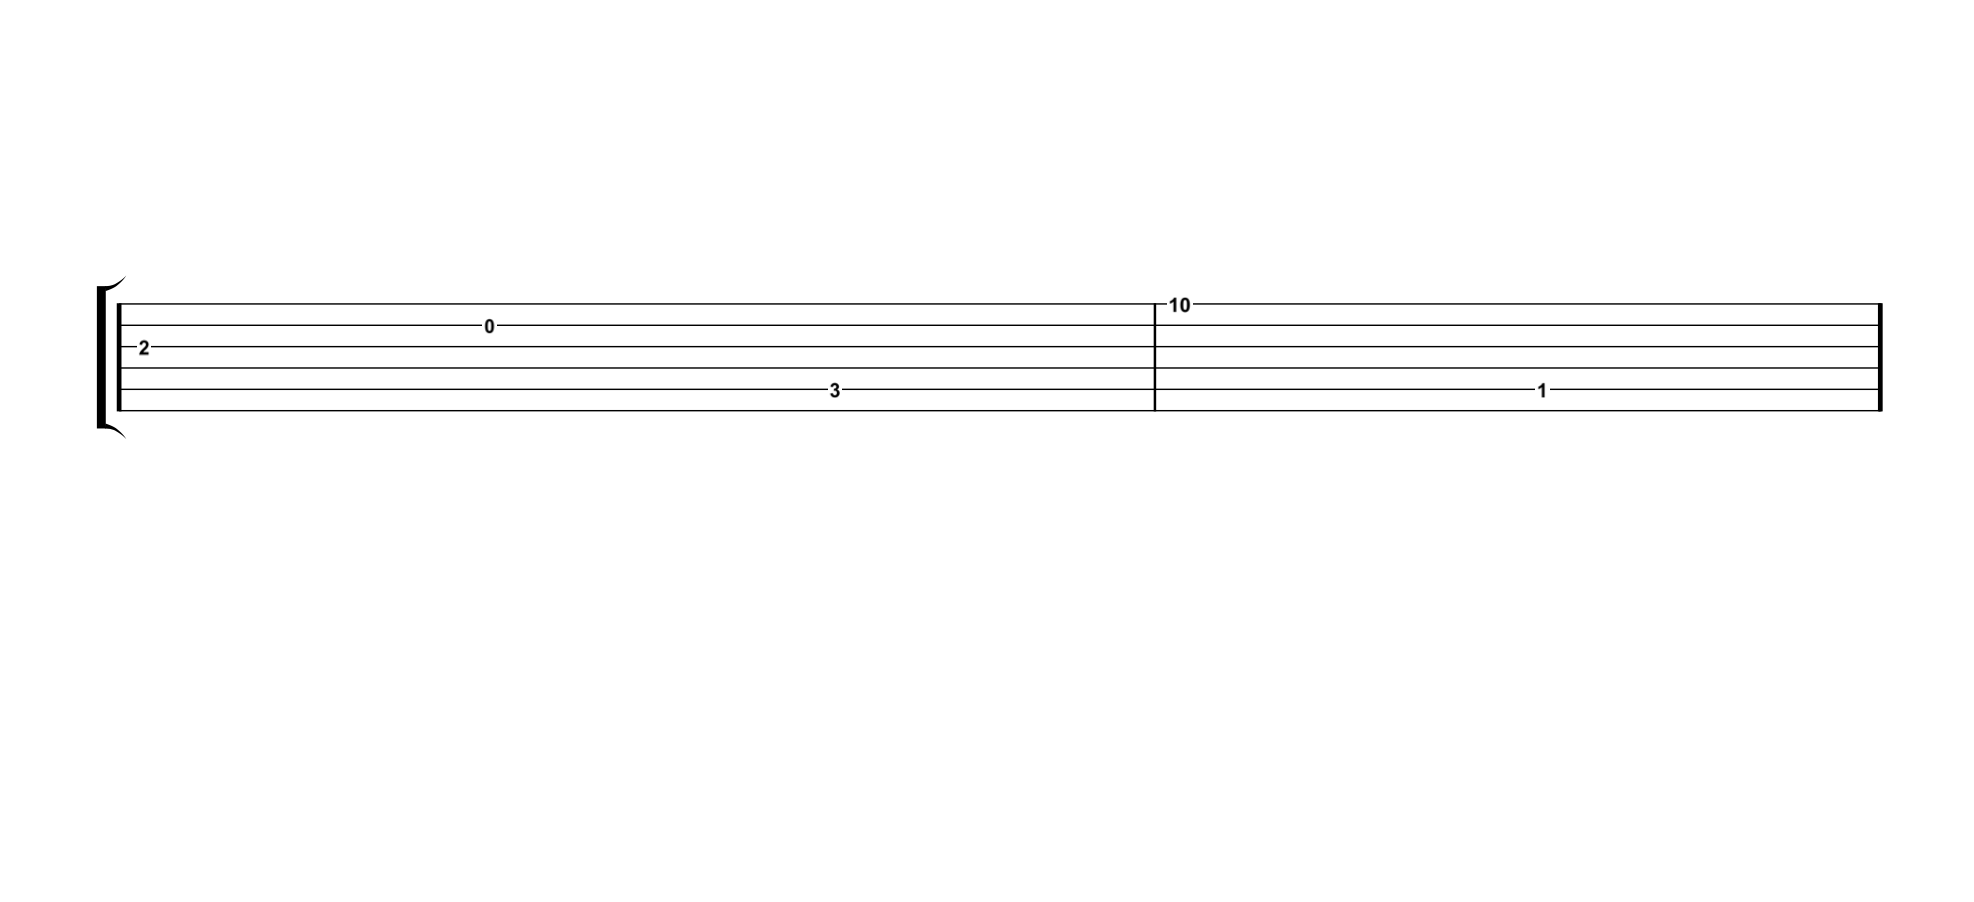
\includegraphics[width=\textwidth]{Minimal}  




\section{Language Concepts}
Data types: \\
There are several data types useful to the user: \\

Notes - consist of a string, pitch, rhythm, and possible properties \\
Measure numbers \\
Specifiers, such as key and time signature \\

Grammar: \\

\begin{verbatim}

<expr>             ::= <option>
                     | <measure>
<option>           ::= <type>
                     | <time>
                     | <key>
<key>              ::= c | cm | c# | c#m| cb | d | dm | db | d#m | e | em | eb | ebm | f | fm | f# | f#m | g | gm | g#m | gb | a | am | a#m | ab | abm | b | bm | bb | bbm
<time>             ::= <num>-<num>
<num>              ::= x ∈ ℕ
<type>             ::= tab
<measure>          ::= <note>+
<note>             ::= <simple>
                     | <complex>
                     | <group>
                     | <tuplet>
<simple>           ::= <singlesimple>
                     | <restsimple>
<complex>          ::= <singlecomplex>
                     | <restcomplex>
<singlesimple>     ::= <string><pitch><property>*
<restsimple>       ::= r
<singlecomplex>    ::= <string><pitch><rhythm><property>*
<restcomplex>      ::= r<rhythm>
<group>            ::= (<singlesimple>+)
                     | (<singlesimple>+)<rhythm>
<tuplet>           ::= t<num>o<num> {<simple>+}
<string>           ::= 1 | 2 | 3 | 4 | 5 | 6
<pitch>            ::= | A | ASharp | AFlat | ANat | B | BSharp | BFlat | BNat | C | CSharp | CFlat | CNat | D | DSharp | DFlat | DNat | E | ESharp | EFlat | ENat | F | FSharp | FFlat | FNat | G | GSharp | GFlat | GNat
<rhythm>           ::= <rhythmnumber><dot>*
<rhythmnumber      ::= 1 | 2 | 4 | 8 | 16 | 32 | 64
<dot>              ::= .
<property>         ::= /sls | /sle | /stu | /std | /p | /plu | /pld | /gr | /har | /sl | /si


\end{verbatim}

\section{Syntax}
A program begins with optional specifiers as to the type of music being written (only tab supported as of now), time signature, and key. They being with a dash, followed by the specifier, and then the actual string \\
e.g.\\
-type tab \\
-key f\# \\
-time 12-8 \\

Measures always being with an int, which is the measure number, followed by a colon \\
e.g. \\
4: \\

Notes start with a string number (1-6), and then a pitch \\
e.g. 5gb \\

A rhythm can be specified as: 1 2 4 8 16 32 64 \\
It can be followed by dots as well \\
e.g. \\
32.. \\
If no rhythm is given, it defaults to 4 \\

Properties can be specified to change or add qualities. They begin with a / and then the abbreviation \\
e.g. \\
/gr means grace note \\

Notes can also be rests, which are an r followed by an optional rhythm \\

Examples of valid notes: \\
5f \\
4g64../gr/sl \\
r \\
r4. \\

This language doesn't really have associativity issues

\section{Semantics}
The table may have floated to another page
\begin{table}[!htbp]
  \begin{center}
    \caption{Data and Operations}
    \label{tab:table1}
    \begin{tabular}{|p{4cm}|p{4cm}|p{4cm}|p{4cm}|}
      \textbf{Syntax} & \textbf{Abstract Syntax} & \textbf{Type} &  \textbf{Meaning} \\
      \hline
      -type tab & ScoreOption of string * string & string * string & This is an option type, where it begins with a dash, followed by the specifier and the data \\ \hline
      1: & measure number & string & A number followed by a colon is the measure number which must precede each measure \\ \hline
      r & RestSimple & Note & An r alone is a simple rest, which uses the default rhythm \\ \hline
      5g\# & SingleSimple of int * Pitch * Property List & Note & This is a simple note, with no rhythm specified, so it uses the default rhythm, which begins as a quarter note and afterwards is whatever the last rhythm specified was. \\ \hline
      4e32/gr & SingleComplex of int * Pitch * Rhythm * PropertyList & Note & This is a complex note, comprised of all the parts that could make up a note \\ \hline
      r32 & RestComplex of Rhythm & Note & This represents a rest, which is complex since it has a rhythm specified
    \end{tabular}
  \end{center}
\end{table}


\section{Remaining Work}
Features that I hope to implement: \\
Dotted rhythms \\
Multiple notes at once \\
Beaming to make rhythms easier to read \\
Decorations, such as slurs, staccatos, slides etc \\
Ability to add title, author name, other text \\

% DO NOT DELETE ANYTHING BELOW THIS LINE
\end{document}
